\documentclass{article}
%
% Demo of the mcode package from 
% http://www.mathworks.co.uk/matlabcentral/fileexchange/8015-m-code-latex-package
% Updated 06 Mar 2014
%

\usepackage{graphicx}
\usepackage{wrapfig}
\usepackage{mathtools}
\usepackage{mathrsfs}
\usepackage{enumitem}
\usepackage{pdflscape}
\graphicspath{ {images/} }

\usepackage{float}
% load package with ``framed'' and ``numbered'' option.
\usepackage[framed,numbered,autolinebreaks,useliterate]{mcode}

% something NOT relevant to the usage of the package.
\usepackage{url}
\setlength{\parindent}{0pt}
\setlength{\parskip}{18pt}


% //////////////////////////////////////////////////

\begin{document}

\title{Homework 10 - Optimal Control Systems}
\author{Erivelton Gualter dos Santos, 2703806}
\date{}

\maketitle 

\section{Stochastic Problem - RC circuit}

The following tables contain the parameters used for this work. The step size is 1ms for 10 s of simulation. The white noise is specified for zero mean and covariance 1e-4. In order to verify the E(J) for numerical and analytical expression, the simulation was executed $1000$ times. It results in a numerical and analytical cost is $0.4884$ and $0.4019$.


\begin{table}[H]
\centering
\caption{Controller parameters}
\label{tb:controller}
\begin{tabular}{|c|c|}
\hline
Parameter & Value \\ \hline \hline
H         & 1     \\ \hline
Q         & 1     \\ \hline
R         & 1     \\ \hline
\end{tabular}
\end{table}

\begin{table}[H]
\centering
\caption{Circuit parameters}
\label{tb:circuit}
\begin{tabular}{|c|c|}
\hline
Parameter & Value \\ \hline
R         & 1     \\ \hline
C         & 1     \\ \hline
\end{tabular}
\end{table}


\begin{figure}[H]
  \centering
  \begin{minipage}[b]{0.45\textwidth}
    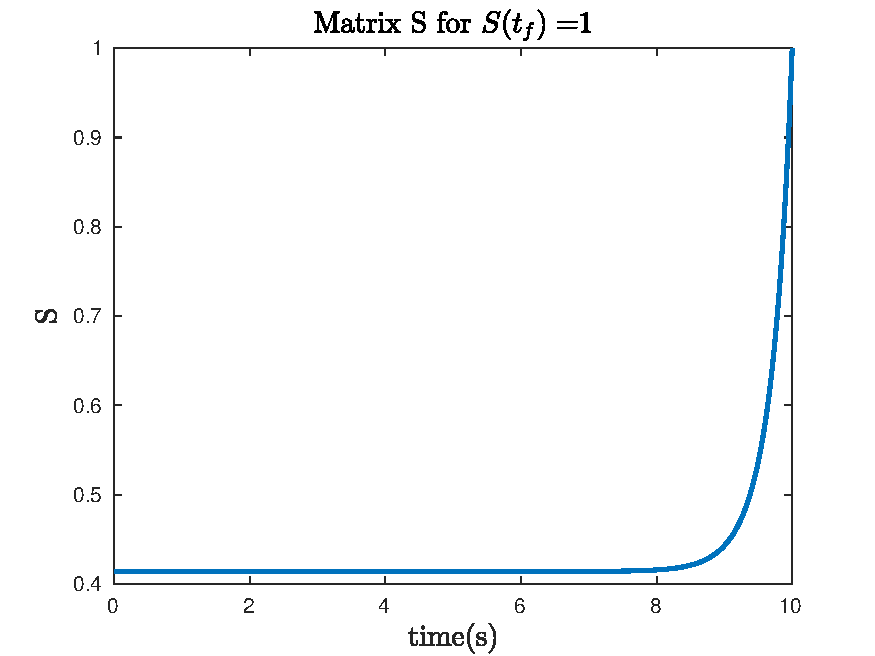
\includegraphics[width=\textwidth]{fig1}
	\caption{Random part.}
  \end{minipage}
  \hfill
  \begin{minipage}[b]{0.45\textwidth}
    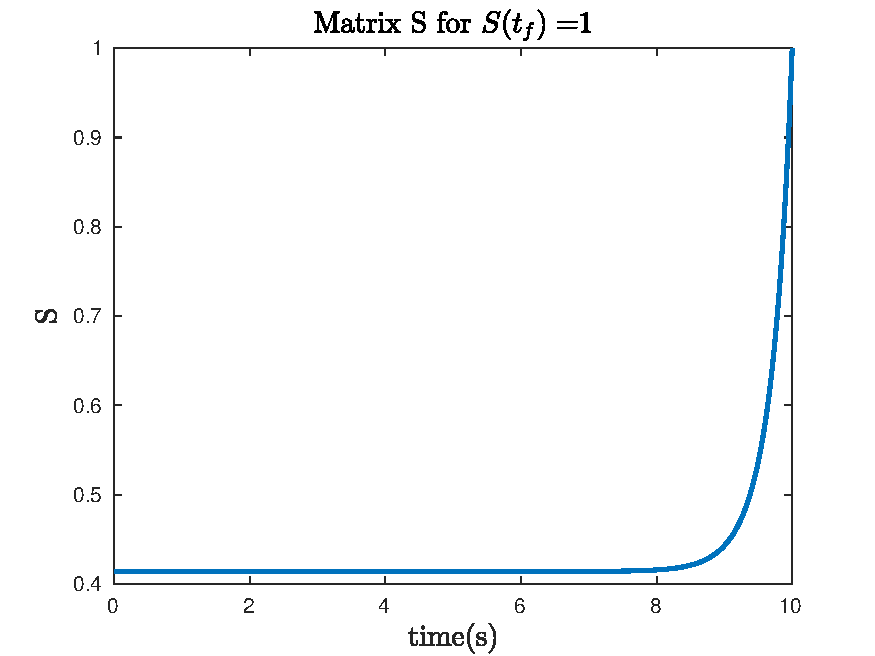
\includegraphics[width=\textwidth]{fig6}
	\caption{Deterministic part.}
  \end{minipage}
\end{figure}

\begin{figure}[H]
  \centering
  \begin{minipage}[b]{0.45\textwidth}
    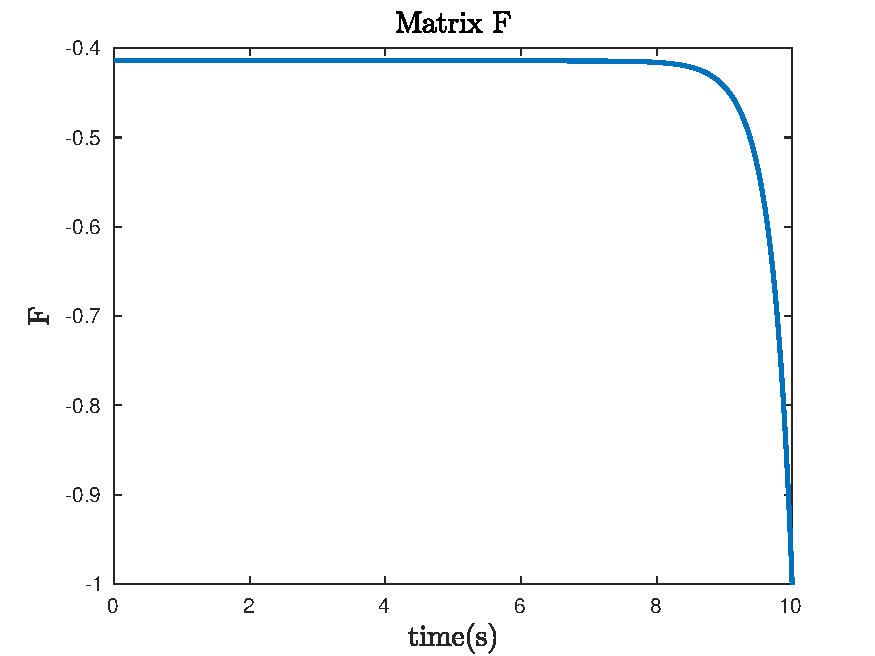
\includegraphics[width=\textwidth]{fig2}
	\caption{Random part.}
  \end{minipage}
  \hfill
  \begin{minipage}[b]{0.45\textwidth}
    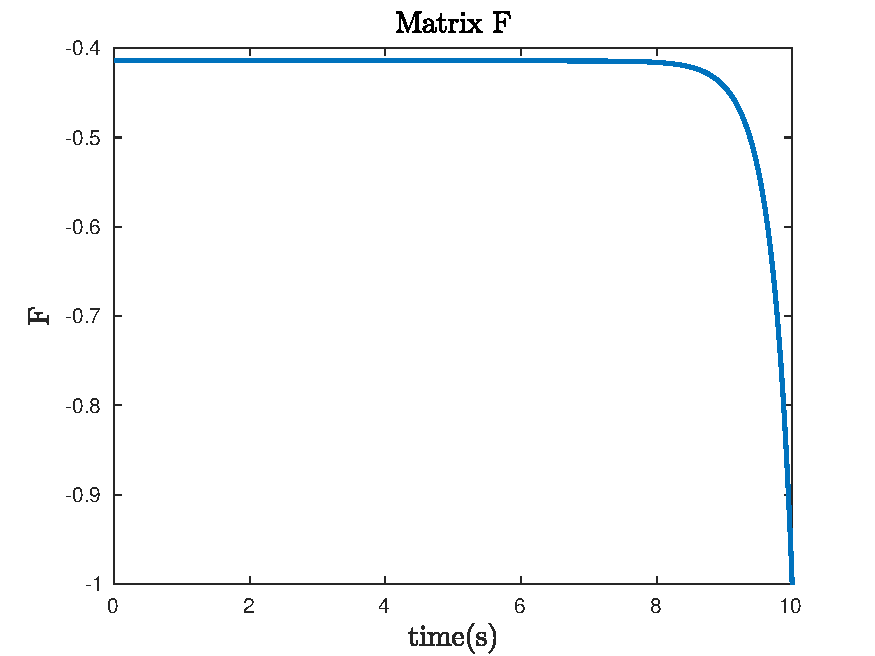
\includegraphics[width=\textwidth]{fig7}
	\caption{Deterministic part.}
  \end{minipage}
\end{figure}

\begin{figure}[H]
  \centering
  \begin{minipage}[b]{0.45\textwidth}
    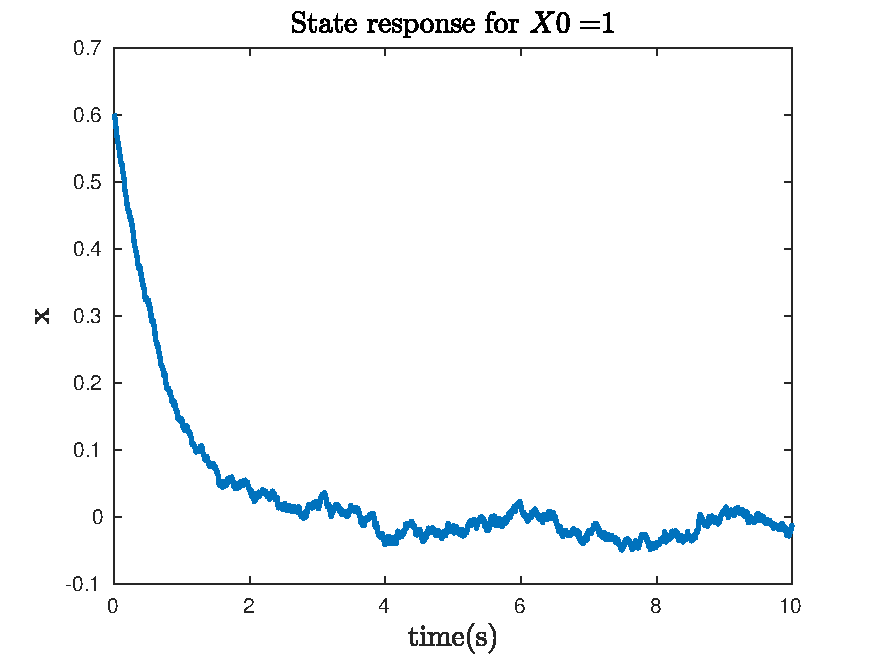
\includegraphics[width=\textwidth]{fig3}
	\caption{Random part.}
  \end{minipage}
  \hfill
  \begin{minipage}[b]{0.45\textwidth}
    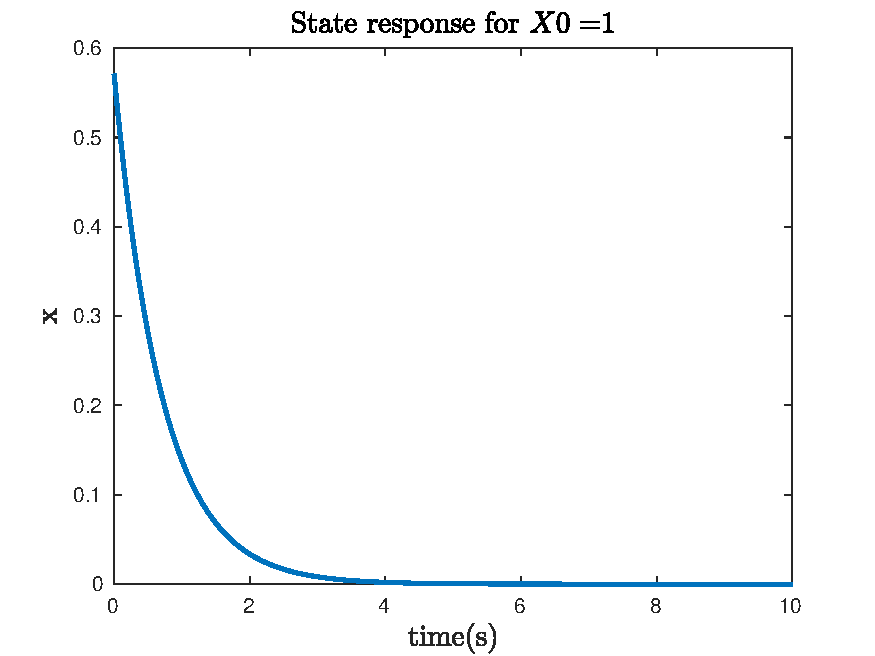
\includegraphics[width=\textwidth]{fig8}
	\caption{Deterministic part.}
  \end{minipage}
\end{figure}

\begin{figure}[H]
  \centering
  \begin{minipage}[b]{0.45\textwidth}
    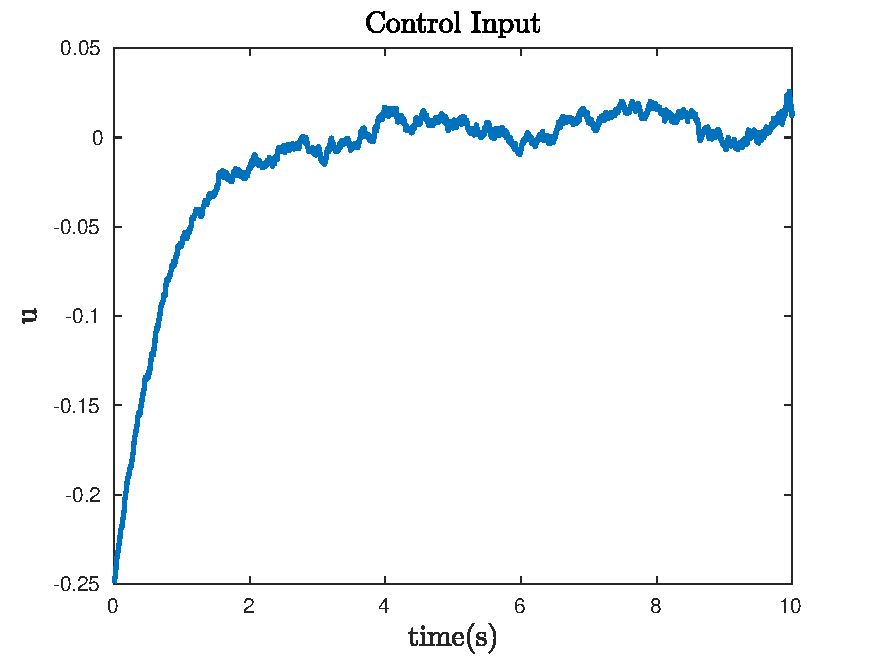
\includegraphics[width=\textwidth]{fig4}
	\caption{Random part.}
  \end{minipage}
  \hfill
  \begin{minipage}[b]{0.45\textwidth}
    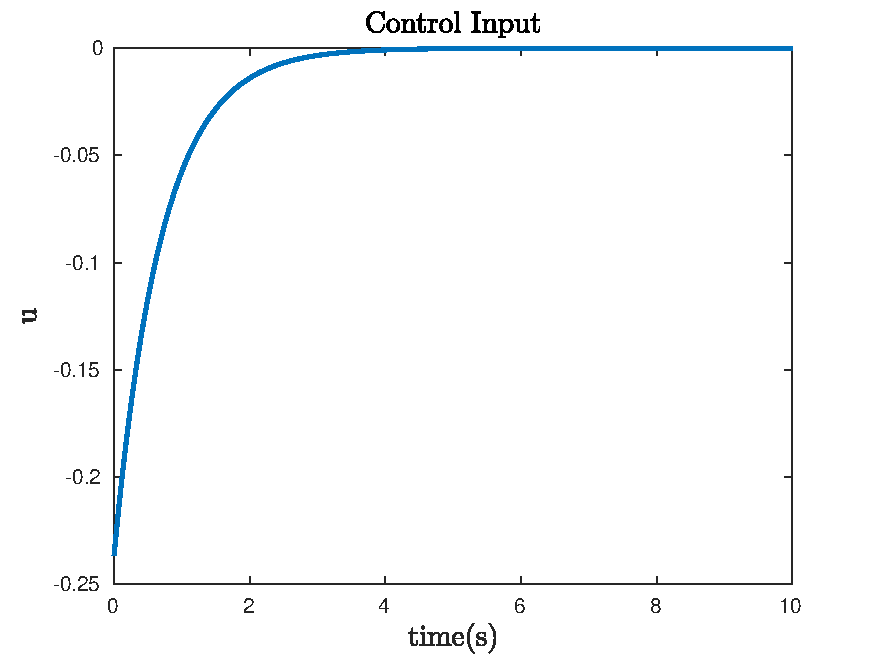
\includegraphics[width=\textwidth]{fig9}
	\caption{Deterministic part.}
  \end{minipage}
\end{figure}

\begin{figure}[H]
  \centering
  \begin{minipage}[b]{0.45\textwidth}
    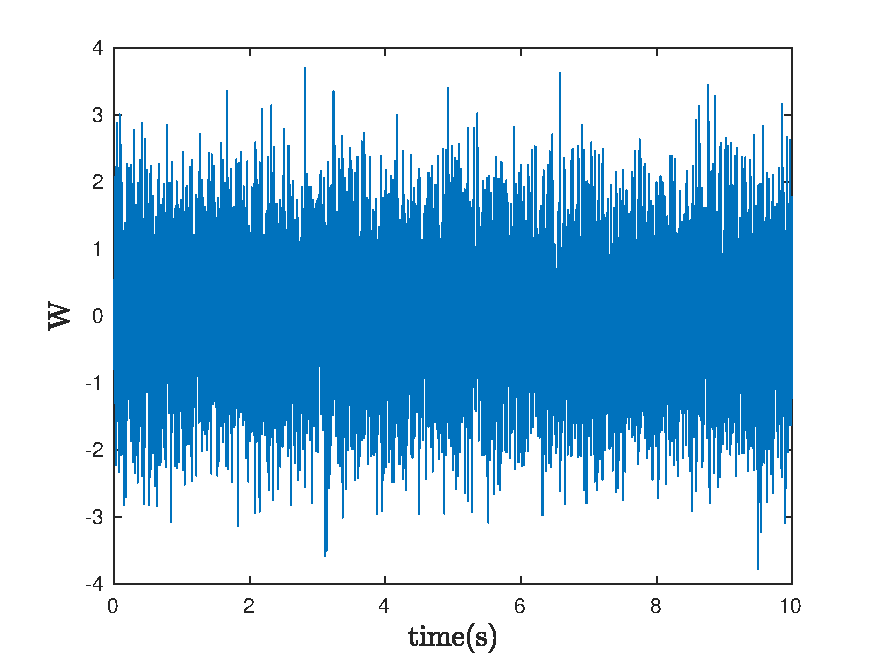
\includegraphics[width=\textwidth]{fig5}
	\caption{Random part.}
  \end{minipage}
  \hfill
  \begin{minipage}[b]{0.45\textwidth}
    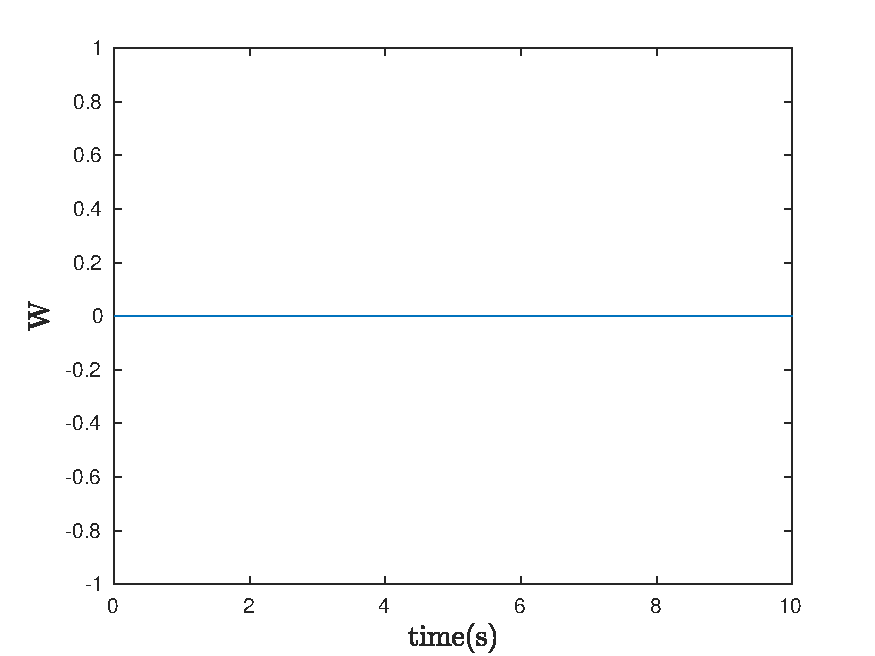
\includegraphics[width=\textwidth]{fig10}
	\caption{Deterministic part.}
  \end{minipage}
\end{figure}


\begin{lstlisting}
% Erivelton Gualter, 04/23/2018

clear all
close all
clc

% Paramters
R = 1;
C = 1;

%state equations
A = -1/(R*C);
B = +1/(R*C);

%Cost function
Q = 1;
R = 1;
H = 1;

dt = 0.001;     % Integration step size
tf = 10;        % Simulation length 
t = 0:dt:tf;    % time array
X0 = 1;         % Initial state
N = round(tf/dt) + 1; %Number of steps

S = zeros(1,N);
S(:,N) = H;
F(N,:)=-inv(R)*B'*S(:,N); 

%Backwards integration in time
for i = 1 : N-1
    SDot = - A'*S(:,N-i+1) - S(:,N-i+1)*A + S(:,N-i+1)*B*inv(R)*B'*S(:,N-i+1) - Q;
    S(:,N-i) = S(:,N-i+1)-SDot*dt;    
    F(N-i,:) = -inv(R)*B'*S(:,N-i);
end

mtimes = 100;       % Number of runs
for k=1:mtimes
    v = 1e-4;       % Covariance
    p0 = 0.1;       % Covariance for Initial Conditions
    X = X0+(p0).^0.5*randn(1,1);

    % System simulation
    for i=1:N
        w(i) = (v/dt).^0.5*randn(1,1);
        u(i) = F(i,:)*X(i);    
        XDot = A*X(i) + B*u(i) + w(i);

        if i < N
            X(i+1) = X(i) + XDot*dt;
        end
    end

    % compute cost
    for j=1:N-1
        xQxuRu(j) = X(:,j)'*Q*X(:,j) + u(j)*R*u(j);
    end

    Jn(k) = X(:,end)'*H*X(:,end) + trapz(t(1:end-1),xQxuRu);
    disp([num2str(k)])
end


mean(Jn) % Numerical cost

% Analytical cost
for j=1:N
    vS(j) = trace(v*S(:,j));
end

disp('Analytical cost')
Ja = trace(S(1)*p0) + trapz(t(1:end),vS(1:end))

%% Plots
close all
f1 = figure;
plot(t, S, 'LineWidth',2);
title(strcat('Matrix S for $S(t_f) =  $', num2str(H)),'Fontsize',14,'interpreter','latex');
xlabel('time(s)', 'Interpreter','Latex', 'FontSize',14);
ylabel('S', 'Interpreter','Latex', 'FontSize',14);

f2 = figure;
plot(t, F, 'LineWidth',2);
title(strcat('Matrix F'), 'Fontsize',14,'interpreter','latex');
xlabel('time(s)', 'Interpreter','Latex', 'FontSize',14);
ylabel('F', 'Interpreter','Latex', 'FontSize',14);

f3 = figure;
plot(t, X, 'LineWidth', 2);
title(strcat('State response for $X0 =  $', num2str(X0)),'Fontsize',14,'interpreter','latex');
xlabel('time(s)', 'Interpreter','Latex', 'FontSize',14);
ylabel('x', 'Interpreter','Latex', 'FontSize',14);

f4 = figure;
plot(t, u, 'LineWidth', 2);
title('Control Input','Fontsize',14,'interpreter','latex');
xlabel('time(s)', 'Interpreter','Latex', 'FontSize',14);
ylabel('u', 'Interpreter','Latex', 'FontSize',14);

f5 = figure;
plot(t, w);
xlabel('time(s)', 'Interpreter','Latex', 'FontSize',14);
ylabel('W', 'Interpreter','Latex', 'FontSize',14);

if v == 0
    saveFigureToPdf('fig6',f1);
    saveFigureToPdf('fig7',f2);
    saveFigureToPdf('fig8',f3);
    saveFigureToPdf('fig9',f4);
    saveFigureToPdf('fig10',f5);
else
    saveFigureToPdf('fig1',f1);
    saveFigureToPdf('fig2',f2);
    saveFigureToPdf('fig3',f3);
    saveFigureToPdf('fig4',f4);
    saveFigureToPdf('fig5',f5);
end
\end{lstlisting}

You can access the code at: https://github.com/EriveltonGualter/EEC-744-Optimal-Control-Systems



\end{document}
